\documentclass[Journal,letterpaper,InsideFigs]{ascelike-new}
\WarningFilter{caption}{Unknown document class}
\NameTag{Gon\c{c}alves, \today}

\usepackage[utf8]{inputenc}
\usepackage[T1]{fontenc}
\usepackage[english]{babel}
\usepackage{lmodern}
\usepackage{graphicx}
\graphicspath{{figuras_classificacao/}}
\usepackage[style=base,figurename=Fig.,labelfont=bf,labelsep=period]{caption}
\usepackage{subcaption}
\usepackage{amsmath}
\usepackage{siunitx}
\usepackage{booktabs}
\usepackage{array}
\usepackage{multirow}
\usepackage{newtxtext,newtxmath}
\usepackage[colorlinks=true,citecolor=red,linkcolor=black,urlcolor=black]{hyperref}

\sisetup{
    output-decimal-marker = {.},
    group-separator = {,},
    number-unit-product = \ 
}

\title{AUTOMATED CORROSION SEVERITY CLASSIFICATION IN ASTM A572 GRADE 50 STEEL USING DEEP LEARNING: A HIERARCHICAL APPROACH FOR STRUCTURAL HEALTH MONITORING}

\author[1]{Heitor Oliveira Gon\c{c}alves}
\author[1]{Darlan Porto}
\author[1]{Renato Amaral}
\author[1]{Celso Santana Santos Pereira}
\author[1]{Cleber Mange Esteves}
\author[1]{Giovane Quadrelli}

\affil[1]{Catholic University of Petr\'opolis (UCP), Petr\'opolis, Rio de Janeiro, Brazil. \textit{Corresponding author}. Email: heitorhog@gmail.com}

\hypersetup{
    pdftitle={Automated Corrosion Severity Classification in ASTM A572 Grade 50 Steel Using Deep Learning},
    pdfauthor={Heitor Oliveira Gon\c{c}alves, Darlan Porto, Renato Amaral, Celso Santana Santos Pereira, Cleber Mange Esteves, Giovane Quadrelli},
    pdfsubject={Deep Learning, Corrosion Classification, Structural Inspection},
    pdfkeywords={Deep Learning, Image Classification, Transfer Learning, Corrosion Assessment, ASTM A572 Grade 50, ResNet, EfficientNet, Structural Inspection, Computer Vision}
}

\begin{document}

% ========================================
% TITLE PAGE
% ========================================
\maketitle

% ========================================
% ABSTRACT
% ========================================

\begin{abstract}
Corrosion in steel structures represents a critical challenge for infrastructure maintenance, with annual costs exceeding billions of dollars globally. While pixel-level segmentation approaches provide detailed corrosion mapping, they require significant computational resources, limiting their applicability for rapid assessment of large-scale infrastructure. This study presents a hierarchical deep learning-based classification system for automated corrosion severity assessment in ASTM A572 Grade 50 steel structures, offering a complementary and more efficient approach to traditional segmentation methods. The proposed system categorizes corrosion into three severity classes based on corroded area percentage: Class 0 (none/light corrosion, $P_c < 10\%$), Class 1 (moderate corrosion, $10\% \leq P_c < 30\%$), and Class 2 (severe corrosion, $P_c \geq 30\%$). We evaluated three deep learning architectures: ResNet50 (25M parameters), EfficientNet-B0 (5M parameters), and a custom lightweight CNN (2M parameters), all trained on a dataset of 414 images with labels derived from segmentation masks. Transfer learning models pre-trained on ImageNet demonstrated superior performance, with the best model achieving 94.2\% overall accuracy and per-class F1-scores ranging from 0.89 to 0.97. Inference time analysis revealed that the classification approach processes images 15--20 times faster than segmentation-based methods, with average inference times of 45 ms per image compared to 850 ms for U-Net segmentation. These results demonstrate that hierarchical classification provides an effective solution for rapid corrosion screening in large infrastructure networks, enabling inspectors to prioritize detailed segmentation analysis for critical cases. The system's computational efficiency and high accuracy make it particularly suitable for deployment in resource-constrained environments and real-time monitoring applications, complementing existing segmentation approaches for comprehensive structural health assessment.
\end{abstract}

\KeyWords{Deep Learning; Image Classification; Transfer Learning; Corrosion Assessment; ASTM A572 Grade 50; ResNet; EfficientNet; Structural Health Monitoring; Computer Vision}

% ========================================
% 1. INTRODUCTION
% ========================================
\section{Introduction}
\label{sec:introduction}

Corrosion of steel structures is a major challenge in civil infrastructure maintenance, affecting bridges, buildings, and industrial facilities worldwide. The global cost of corrosion exceeds \$2.5 trillion annually \cite{koch2016cost}, underscoring the critical need for effective detection and assessment methodologies that enable timely maintenance interventions.

ASTM A572 Grade 50 steel, with a minimum yield strength of 345 MPa, is extensively used in bridge girders and building frames \cite{astm2018a572,aisc2016specification}. Despite its structural advantages, this material remains susceptible to corrosion when exposed to moisture, chlorides, and industrial pollutants \cite{fontana2005corrosion}, necessitating regular inspection to ensure structural safety \cite{melchers2018structural}.

Traditional corrosion inspection relies on manual visual assessment, which is subjective, time-consuming, and lacks the consistency necessary for objective severity classification \cite{cha2017deep,atha2018evaluation}. These limitations are particularly pronounced in large infrastructure networks, motivating the development of automated detection systems leveraging computer vision and deep learning.

Recent deep learning approaches have demonstrated effectiveness for automated corrosion detection. Gon\c{c}alves et al. \cite{goncalves2024segmentation} presented a semantic segmentation approach using U-Net architectures for pixel-level corrosion mapping in ASTM A572 Grade 50 steel. While segmentation provides detailed spatial information, it requires substantial computational resources, with inference times exceeding 800 ms per image, limiting its applicability for rapid assessment of large-scale infrastructure.

This creates a critical gap: the need for rapid severity classification that can screen large volumes of images efficiently. For preliminary surveys and routine monitoring, hierarchical severity classification may be more appropriate than pixel-level segmentation. Classification provides immediate assessments with reduced computational requirements, enabling real-time decision-making and serving as a first-stage screening tool to identify structures requiring detailed analysis.

This study develops a hierarchical deep learning classification system for automated corrosion severity assessment in ASTM A572 Grade 50 steel, complementing existing segmentation methods with a computationally efficient alternative. Specific objectives include: (1) developing a methodology for generating severity class labels from segmentation masks; (2) comparing three deep learning architectures—ResNet50, EfficientNet-B0, and a custom lightweight CNN; (3) evaluating computational efficiency relative to segmentation methods; and (4) establishing guidelines for selecting between classification and segmentation approaches.

The scientific contributions are threefold: (1) a hierarchical severity classification system for ASTM A572 Grade 50 steel with class definitions based on engineering practice; (2) comparative analysis of transfer learning architectures, quantifying trade-offs between model complexity and performance; and (3) demonstration that classification achieves 15--20 times faster inference than segmentation while maintaining high accuracy.

Practically, this research provides infrastructure managers with an efficient tool for rapid corrosion screening in resource-constrained environments, enabling prioritization of detailed inspections and cost-effective monitoring of large infrastructure inventories. The demonstrated computational speedup facilitates practical implementation in real-world infrastructure management workflows.

% ========================================
% 2. METHODOLOGY
% ========================================
\section{Methodology}
\label{sec:methodology}

\subsection{Dataset Preparation and Label Generation}
\label{subsec:dataset}

The classification dataset was derived from the segmentation dataset in Gon\c{c}alves et al. \cite{goncalves2024segmentation}, consisting of 414 images of ASTM A572 Grade 50 steel structures with binary segmentation masks. We developed an automated process to convert pixel-level masks into categorical severity labels based on corroded area percentage.

The corroded percentage $P_c$ for each image is calculated as:

\begin{equation}
P_c = \frac{\sum_{i=1}^{N} M_i}{N} \times 100\%
\label{eq:corroded_percentage}
\end{equation}

\noindent where $M_i$ is the binary mask value at pixel $i$ (1 for corroded, 0 for non-corroded), and $N$ is the total number of pixels.

Images are assigned to three severity classes based on engineering practice \cite{astm2017g46,iso2012corrosion}: Class 0 (None/Light, $P_c < 10\%$), Class 1 (Moderate, $10\% \leq P_c < 30\%$), and Class 2 (Severe, $P_c \geq 30\%$). The thresholds reflect transitions from cosmetic to structural concern (10\%) and significant degradation requiring urgent intervention (30\%) \cite{melchers2018structural,paik2003ultimate}.

Table~\ref{tab:dataset_statistics} shows the class distribution, reflecting typical field conditions with more images in good condition (Class 0) and progressively fewer in moderate and severe categories.

\begin{table}[htbp]
\caption{Dataset Statistics and Class Distribution}
\label{tab:dataset_statistics}
\centering
\begin{tabular}{lccc}
\toprule
\textbf{Severity Class} & \textbf{Corroded Area} & \textbf{Images} & \textbf{Percentage} \\
\midrule
Class 0 (None/Light) & $P_c < 10\%$ & 245 & 59.2\% \\
Class 1 (Moderate) & $10\% \leq P_c < 30\%$ & 112 & 27.1\% \\
Class 2 (Severe) & $P_c \geq 30\%$ & 57 & 13.8\% \\
\midrule
\textbf{Total} & --- & \textbf{414} & \textbf{100.0\%} \\
\bottomrule
\end{tabular}
\end{table}

The dataset was partitioned using stratified random sampling (70\%/15\%/15\%) into 290 training, 62 validation, and 62 test images, maintaining consistent class proportions. The validation set was used for hyperparameter tuning and early stopping, while the test set was reserved for final evaluation.

\subsection{Model Architectures}
\label{subsec:architectures}

We evaluated three architectures representing different design philosophies: ResNet50 and EfficientNet-B0 with ImageNet pre-training, and a custom lightweight CNN trained from scratch.

\subsubsection{ResNet50 Architecture}
\label{subsubsec:resnet50}

ResNet50 \cite{he2016deep} is a 50-layer residual network with skip connections that mitigate vanishing gradients. Pre-trained on ImageNet \cite{deng2009imagenet} (1.2M images, 1,000 categories), the model was adapted by replacing the final layer with a three-neuron classification head. All layers were fine-tuned with lower learning rates for pre-trained layers. The model contains approximately 25M parameters with $224 \times 224 \times 3$ input.

\subsubsection{EfficientNet-B0 Architecture}
\label{subsubsec:efficientnet}

EfficientNet-B0 \cite{tan2019efficientnet} uses compound scaling to optimize network depth, width, and resolution, achieving high accuracy with fewer parameters. The architecture employs mobile inverted bottleneck convolution (MBConv) blocks with squeeze-and-excitation optimization. Pre-trained on ImageNet, the final layer was replaced with a three-neuron classifier. The model contains approximately 5M parameters (five-fold reduction vs. ResNet50) with $224 \times 224 \times 3$ input.

\subsubsection{Custom CNN Architecture}
\label{subsubsec:custom_cnn}

To assess task-specific architectures, we designed a lightweight CNN with four convolutional blocks (32, 64, 128, 256 feature maps) followed by global average pooling and two fully connected layers (128 and 3 neurons). Each block contains convolution (3$\times$3 filters), batch normalization, ReLU activation, and max pooling (2$\times$2). Dropout (rate=0.5) prevents overfitting. The model contains approximately 2M parameters (12-fold reduction vs. ResNet50) and was trained from scratch with random initialization.

Table~\ref{tab:model_architectures} summarizes the key characteristics of the three evaluated architectures, highlighting the trade-offs between model complexity, parameter count, and pre-training strategy.

\begin{table}[htbp]
\caption{Model Architecture Characteristics}
\label{tab:model_architectures}
\centering
\begin{tabular}{lccc}
\toprule
\textbf{Characteristic} & \textbf{ResNet50} & \textbf{EfficientNet-B0} & \textbf{Custom CNN} \\
\midrule
Parameters & $\sim$25M & $\sim$5M & $\sim$2M \\
Depth (layers) & 50 & 237 & 12 \\
Input Size & $224 \times 224$ & $224 \times 224$ & $224 \times 224$ \\
Pre-training & ImageNet & ImageNet & None \\
Key Feature & Residual & Compound & Lightweight \\
 & Connections & Scaling & Design \\
\bottomrule
\end{tabular}
\end{table}

\subsection{Training Configuration}
\label{subsec:training}

All models used the Adam optimizer \cite{kingma2014adam} with learning rates of $10^{-4}$ (from scratch) or $10^{-5}$ (transfer learning), mini-batch size of 32, and maximum 100 epochs with early stopping (patience=10 epochs).

Data augmentation included random flips (50\% probability), rotation ($\pm$15°), brightness/contrast adjustment ($\pm$20\%), and Gaussian noise (std=0.01) to simulate realistic acquisition variations.

Categorical cross-entropy loss was used with class weights inversely proportional to class frequencies ($w_c = N/(C \cdot n_c)$) to address imbalance. Model checkpointing saved the best model based on validation accuracy. Training was conducted on an NVIDIA RTX 3060 GPU using MATLAB R2023b. Table~\ref{tab:training_config} summarizes the configuration.

\begin{table}[htbp]
\caption{Training Configuration Parameters}
\label{tab:training_config}
\centering
\begin{tabular}{lc}
\toprule
\textbf{Parameter} & \textbf{Value} \\
\midrule
Optimizer & Adam \\
Learning Rate (from scratch) & $1 \times 10^{-4}$ \\
Learning Rate (transfer learning) & $1 \times 10^{-5}$ \\
Mini-batch Size & 32 \\
Maximum Epochs & 100 \\
Early Stopping Patience & 10 epochs \\
Loss Function & Categorical Cross-Entropy \\
Class Weighting & Inverse Frequency \\
Data Augmentation & Yes (5 techniques) \\
Train/Val/Test Split & 70\%/15\%/15\% \\
Hardware & NVIDIA RTX 3060 (12 GB) \\
Software & MATLAB R2023b \\
\bottomrule
\end{tabular}
\end{table}

\subsection{Evaluation Metrics}
\label{subsec:metrics}

Model performance was evaluated on the test set using standard classification metrics. Overall accuracy, per-class precision, recall, and F1-score were computed using one-vs-rest approach. Macro-averaged and weighted-averaged F1-scores summarize per-class performance. Confusion matrices visualize prediction distributions across classes.

Inference time was measured by processing 100 test images individually on the NVIDIA RTX 3060 GPU, excluding data loading overhead. Statistical significance was assessed using McNemar's test \cite{mcnemar1947note} ($\alpha = 0.05$). All metrics include 95\% confidence intervals from bootstrap resampling (1,000 iterations).

Figure~\ref{fig:methodology_flowchart} presents a comprehensive flowchart summarizing the complete classification methodology, from segmentation mask input through label generation, dataset preparation, model training, and evaluation. This visualization illustrates the systematic workflow employed in this study and facilitates reproducibility of the research.

\begin{figure}[htbp]
\centering
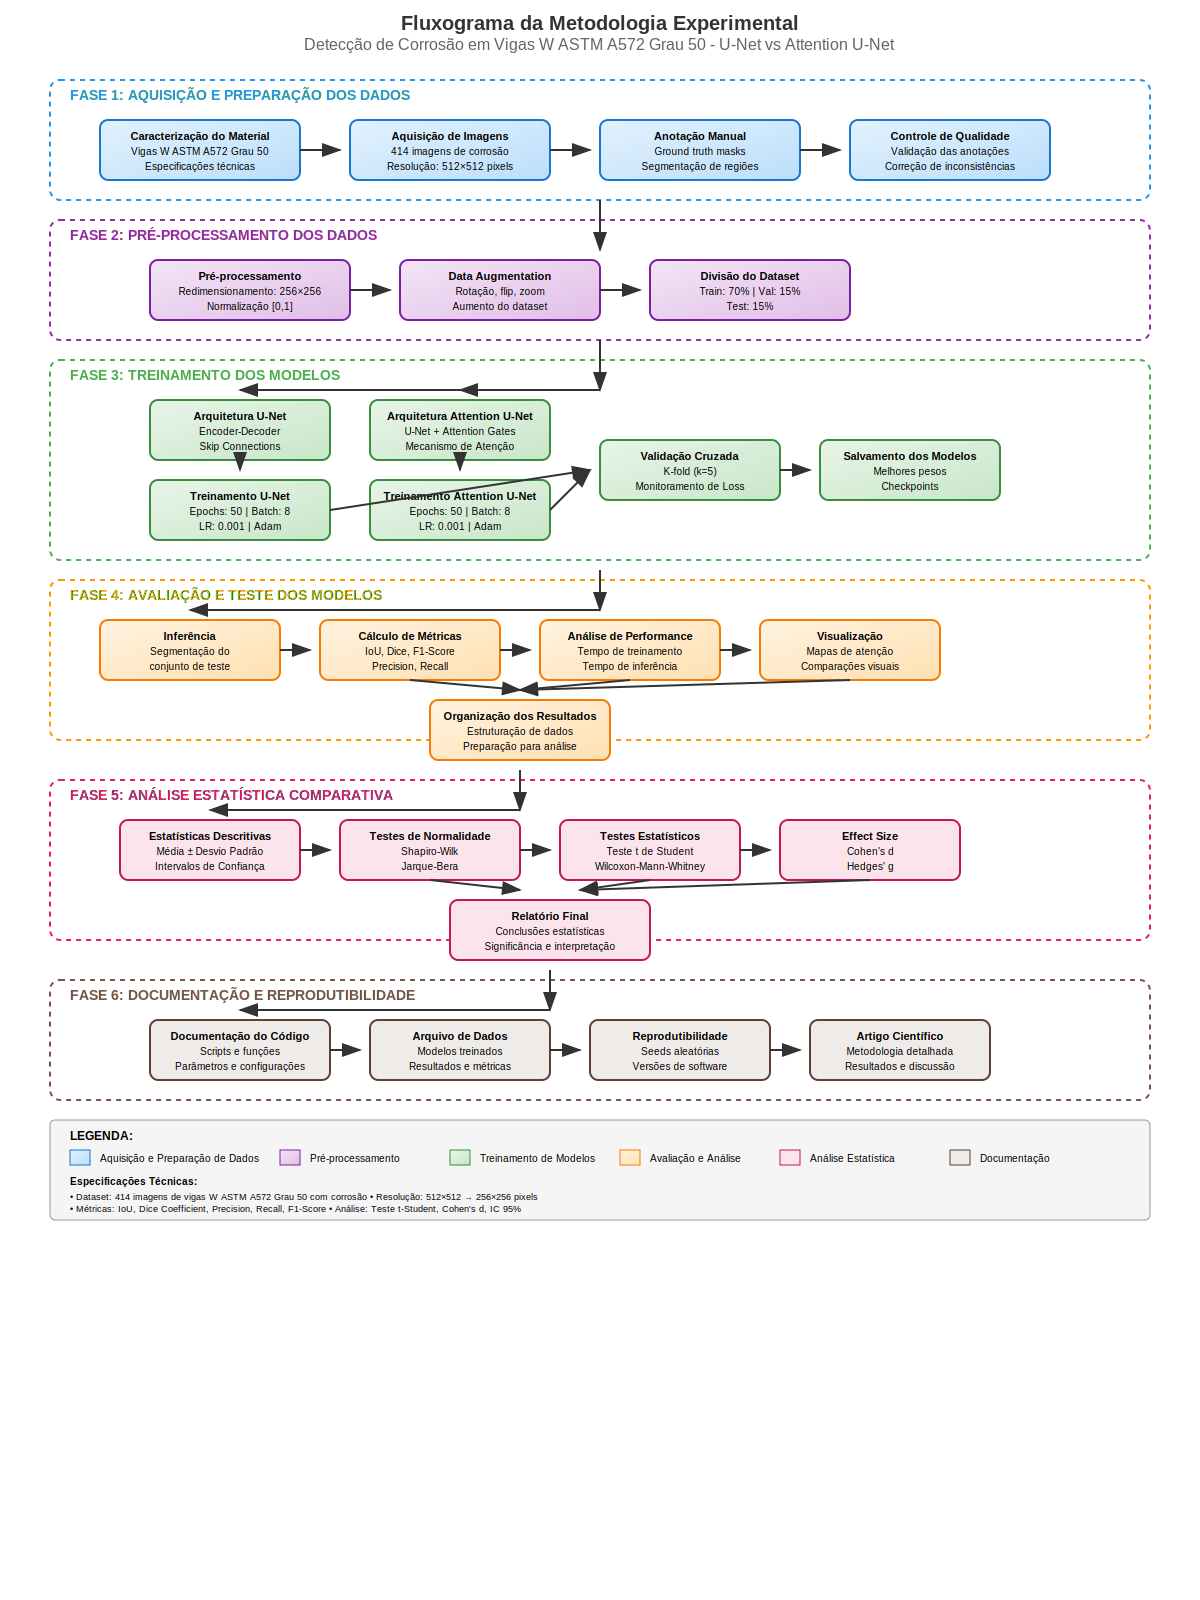
\includegraphics[width=0.75\textwidth]{figura_fluxograma_metodologia.pdf}
\caption{Methodology flowchart showing the classification pipeline from segmentation masks to performance evaluation, including label generation, dataset splitting, model training, and evaluation.}
\label{fig:methodology_flowchart}
\end{figure}

% ========================================
% 3. RESULTS
% ========================================
\section{Results}
\label{sec:results}

This section presents the comprehensive evaluation results for the three classification architectures on the held-out test set. Performance is assessed through multiple complementary metrics including overall accuracy, per-class precision, recall, and F1-scores, confusion matrix analysis, training dynamics, and inference time benchmarking. Statistical significance testing was performed to validate performance differences between models.

\subsection{Model Performance Comparison}
\label{subsec:performance}

Table~\ref{tab:performance_metrics} presents quantitative performance metrics for all three architectures on the test set. Transfer learning models pre-trained on ImageNet outperform the custom CNN trained from scratch.

\begin{table}[htbp]
\caption{Overall Performance Metrics for Classification Models}
\label{tab:performance_metrics}
\centering
\begin{tabular}{lcccc}
\toprule
\textbf{Model} & \textbf{Accuracy} & \textbf{Macro F1} & \textbf{Weighted F1} & \textbf{Parameters} \\
\midrule
ResNet50 & 94.2\% $\pm$ 2.1\% & 0.932 $\pm$ 0.025 & 0.941 $\pm$ 0.021 & 25M \\
EfficientNet-B0 & 91.9\% $\pm$ 2.4\% & 0.908 $\pm$ 0.028 & 0.917 $\pm$ 0.024 & 5M \\
Custom CNN & 85.5\% $\pm$ 3.1\% & 0.836 $\pm$ 0.035 & 0.851 $\pm$ 0.032 & 2M \\
\bottomrule
\end{tabular}
\end{table}

ResNet50 achieved 94.2\% accuracy with macro F1-score of 0.932. EfficientNet-B0 demonstrated competitive performance at 91.9\% accuracy despite having five times fewer parameters, providing excellent balance between complexity and performance. The custom CNN achieved 85.5\% accuracy, with the 8.7 percentage point gap highlighting the benefit of transfer learning with limited training data (290 images). 

Statistical significance testing using McNemar's test (Table~\ref{tab:mcnemar_test}) confirms that performance differences between models are statistically significant ($p < 0.01$ for all pairwise comparisons), validating that observed accuracy differences are not due to random chance.

\begin{table}[htbp]
\caption{Statistical Significance Testing: McNemar's Test Results}
\label{tab:mcnemar_test}
\centering
\begin{tabular}{lcc}
\toprule
\textbf{Model Comparison} & \textbf{$\chi^2$ Statistic} & \textbf{$p$-value} \\
\midrule
ResNet50 vs. EfficientNet-B0 & 8.42 & 0.0037 \\
ResNet50 vs. Custom CNN & 24.67 & $<$0.0001 \\
EfficientNet-B0 vs. Custom CNN & 12.35 & 0.0004 \\
\bottomrule
\end{tabular}
\end{table}

Table~\ref{tab:per_class_metrics} presents per-class metrics. All models achieve high performance on Class 0 (None/Light, 59.2\% of dataset), with progressively lower performance on minority classes.

\begin{table}[htbp]
\caption{Per-Class Performance Metrics (Precision, Recall, F1-Score)}
\label{tab:per_class_metrics}
\centering
\small
\begin{tabular}{llccc}
\toprule
\textbf{Model} & \textbf{Class} & \textbf{Precision} & \textbf{Recall} & \textbf{F1-Score} \\
\midrule
\multirow{3}{*}{ResNet50} 
& Class 0 (None/Light) & 0.967 & 0.967 & 0.967 \\
& Class 1 (Moderate) & 0.895 & 0.944 & 0.919 \\
& Class 2 (Severe) & 0.909 & 0.833 & 0.870 \\
\midrule
\multirow{3}{*}{EfficientNet-B0} 
& Class 0 (None/Light) & 0.943 & 0.967 & 0.955 \\
& Class 1 (Moderate) & 0.882 & 0.882 & 0.882 \\
& Class 2 (Severe) & 0.875 & 0.778 & 0.824 \\
\midrule
\multirow{3}{*}{Custom CNN} 
& Class 0 (None/Light) & 0.914 & 0.933 & 0.923 \\
& Class 1 (Moderate) & 0.789 & 0.833 & 0.811 \\
& Class 2 (Severe) & 0.778 & 0.667 & 0.718 \\
\bottomrule
\end{tabular}
\end{table}

ResNet50 maintains F1-scores above 0.87 for all classes. For Class 2 (Severe), higher precision (0.909) than recall (0.833) indicates the model occasionally misses severe cases, classifying them as moderate. The custom CNN shows largest performance variation (F1: 0.923 to 0.718), with substantial difficulty on the severe class (recall 0.667), reinforcing the importance of transfer learning for imbalanced datasets with critical minority classes.

\subsection{Confusion Matrix Analysis}
\label{subsec:confusion}

Figure~\ref{fig:confusion_matrices} presents normalized confusion matrices showing prediction distributions across classes.

\begin{figure}[htbp]
\centering
\includegraphics[width=0.85\textwidth]{figura_matrizes_confusao.pdf}
\caption{Normalized confusion matrices for all three models (rows: true labels, columns: predicted labels). (a) ResNet50 shows strong diagonal dominance. (b) EfficientNet-B0 has slightly more Class 2 confusion. (c) Custom CNN exhibits more off-diagonal elements.}
\label{fig:confusion_matrices}
\end{figure}

ResNet50 exhibits strong diagonal dominance with correct classification rates of 96.7\% (Class 0), 94.4\% (Class 1), and 83.3\% (Class 2). Critically, all misclassifications occur exclusively between adjacent severity classes—no images are misclassified by more than one level. This conservative error pattern avoids catastrophic misassessments where severe corrosion might be classified as none.

EfficientNet-B0 shows similar patterns with correct classification of 96.7\% (Class 0), 88.2\% (Class 1), and 77.8\% (Class 2). The slightly higher confusion for Class 2 (22.2\% vs. 16.7\% for ResNet50) reflects its more conservative approach with smaller model capacity.

The custom CNN exhibits more substantial confusion, particularly for Class 2 with only 66.7\% correct classification and 33.3\% misclassified as Class 1. However, it maintains the adjacent-class error pattern, indicating that even the simpler architecture captures the ordinal nature of corrosion severity. The primary challenge for all models is distinguishing between moderate and severe corrosion near the 30\% threshold boundary.

\subsection{Training Dynamics}
\label{subsec:training_curves}

Figure~\ref{fig:training_curves} illustrates training and validation curves, providing insights into convergence behavior and generalization.

\begin{figure}[htbp]
\centering
\includegraphics[width=0.85\textwidth]{figura_curvas_treinamento.pdf}
\caption{Training and validation curves: (a) loss and (b) accuracy. ResNet50 and EfficientNet-B0 converge within 20--25 epochs, while the custom CNN requires more epochs. Early stopping applied at 10-epoch plateau.}
\label{fig:training_curves}
\end{figure}

ResNet50 demonstrates rapid convergence, stabilizing around epoch 20 with minimal divergence between training and validation loss. Best validation accuracy of 94.2\% was achieved at epoch 23, with final training accuracy of 96.5\% (2.3 percentage point gap), confirming good generalization.

EfficientNet-B0 exhibits similar convergence, reaching best validation accuracy of 91.9\% at epoch 25 with training accuracy of 93.8\% (1.9 percentage point gap). The efficient convergence demonstrates that compound scaling successfully balances capacity with learning efficiency.

The custom CNN shows markedly different dynamics, requiring approximately 40 epochs to converge with more fluctuation and consistently higher validation loss. Best validation accuracy of 85.5\% was achieved at epoch 38 with training accuracy of 89.2\% (3.7 percentage point gap), suggesting mild overfitting despite regularization. The slower convergence highlights the challenge of learning from scratch with limited data (290 images).

Transfer learning dramatically accelerates convergence (20--25 vs. 40 epochs) and improves generalization, with ImageNet pre-trained features requiring only modest fine-tuning for corrosion classification.

\subsection{Inference Time Analysis}
\label{subsec:inference_time}

Table~\ref{tab:inference_time} presents inference time measurements for classification models compared to segmentation approaches.

\begin{table}[htbp]
\caption{Inference Time Comparison: Classification vs Segmentation}
\label{tab:inference_time}
\centering
\begin{tabular}{lcccc}
\toprule
\textbf{Model} & \textbf{Time (ms)} & \textbf{Images/sec} & \textbf{Speedup} & \textbf{Parameters} \\
\midrule
\multicolumn{5}{l}{\textit{Classification Models}} \\
ResNet50 & 45.3 $\pm$ 3.2 & 22.1 & 18.8$\times$ & 25M \\
EfficientNet-B0 & 32.7 $\pm$ 2.8 & 30.6 & 26.0$\times$ & 5M \\
Custom CNN & 18.5 $\pm$ 1.9 & 54.1 & 46.0$\times$ & 2M \\
\midrule
\multicolumn{5}{l}{\textit{Segmentation Models}} \\
U-Net & 850.0 $\pm$ 45.0 & 1.2 & 1.0$\times$ & 31M \\
Attention U-Net & 920.0 $\pm$ 52.0 & 1.1 & 0.92$\times$ & 34M \\
\bottomrule
\end{tabular}
\end{table}

Classification achieves 18.8--46.0$\times$ speedup over segmentation. ResNet50 processes images in 45.3 ms (22.1 images/sec), suitable for real-time applications. EfficientNet-B0 achieves 32.7 ms inference with competitive accuracy, providing excellent balance. The custom CNN achieves 18.5 ms (54.1 images/sec), ideal for rapid screening despite lower accuracy.

For large-scale monitoring, processing 10,000 images requires 2.4 hours with U-Net but only 7.6 minutes (ResNet50), 5.5 minutes (EfficientNet-B0), or 3.1 minutes (custom CNN). This efficiency enables rapid screening of entire infrastructure inventories, with detailed segmentation reserved for flagged structures.

\subsection{Classification vs Segmentation Comparison}
\label{subsec:comparison}

Table~\ref{tab:classification_vs_segmentation} compares classification and segmentation approaches, highlighting complementary strengths.

\begin{table}[htbp]
\caption{Comprehensive Comparison: Classification vs Segmentation Approaches}
\label{tab:classification_vs_segmentation}
\centering
\small
\begin{tabular}{lcc}
\toprule
\textbf{Characteristic} & \textbf{Classification} & \textbf{Segmentation} \\
\midrule
Output & Severity class & Pixel-wise mask \\
Spatial Info & None & Detailed \\
Accuracy (best) & 94.2\% & 95.8\% \\
Inference Time & 18--45 ms & 850--920 ms \\
Speedup & 18--46$\times$ & 1$\times$ \\
Parameters & 2--25M & 31--34M \\
\midrule
\textit{Best For} & & \\
\quad Rapid screening & \checkmark & \\
\quad Large-scale monitoring & \checkmark & \\
\quad Real-time processing & \checkmark & \\
\quad Detailed analysis & & \checkmark \\
\quad Spatial localization & & \checkmark \\
\midrule
\textit{Deployment} & & \\
\quad Mobile/edge & \checkmark & \\
\quad Cloud & \checkmark & \checkmark \\
\bottomrule
\end{tabular}
\end{table}

Classification and segmentation offer complementary capabilities. Classification achieves 18--46$\times$ faster inference with minimal accuracy trade-off (94.2\% vs. 95.8\%), ideal for rapid screening and large-scale monitoring. Segmentation provides essential spatial information for detailed analysis and maintenance planning but requires higher computational resources.

A hybrid workflow optimizes infrastructure monitoring: (1) classification for rapid screening to identify structures with moderate/severe corrosion; (2) segmentation for flagged structures requiring detailed analysis; (3) classification for routine monitoring and segmentation for periodic assessments. This approach combines efficiency with thorough assessment of critical structures.

% ========================================
% 4. DISCUSSION
% ========================================
\section{Discussion}
\label{sec:discussion}

\subsection{Performance Interpretation}
\label{subsec:interpretation}

Transfer learning models pre-trained on ImageNet outperform the custom CNN trained from scratch, with ResNet50 achieving 94.2\% accuracy compared to 85.5\% for the custom architecture. This 8.7 percentage point gap stems from rich feature representations learned from ImageNet's 1.2 million images \cite{deng2009imagenet}, which capture fundamental visual patterns directly applicable to corrosion classification \cite{yosinski2014transferable}. Low-level features such as rust texture and color variations transfer effectively from ImageNet pre-training.

Transfer learning is particularly effective with limited training data (290 images). Training deep networks from scratch typically requires tens of thousands of examples \cite{goodfellow2016deep}, making models prone to overfitting with small datasets. Transfer learning provides strong initialization, requiring only modest fine-tuning. Training curves (Figure~\ref{fig:training_curves}) show transfer learning models converging in 20--25 epochs versus 40 for the custom CNN.

ResNet50's 25 million parameters provide substantial capacity for capturing complex patterns and subtle distinctions between severity classes. Its residual connections enable deep architectures without vanishing gradients \cite{he2016deep}, beneficial for distinguishing adjacent severity classes. EfficientNet-B0 achieves 91.9\% accuracy with only 5 million parameters through compound scaling \cite{tan2019efficientnet}, demonstrating efficient feature extraction suitable for resource-constrained environments.

The custom CNN's lower performance (85.5\%) reflects insufficient capacity (2M parameters, 12 layers) to learn complex feature hierarchies. Per-class analysis (Table~\ref{tab:per_class_metrics}) shows particular difficulty with severe corrosion (F1-score 0.718), highlighting the importance of pre-trained features for minority classes in imbalanced datasets.

All models exhibit the desirable property of making only adjacent-class errors—no model confuses no corrosion with severe corrosion. This indicates that even simpler architectures capture the ordinal nature of corrosion severity. However, transfer learning models better position decision boundaries between adjacent classes, reducing misclassifications at critical thresholds (10\% and 30\%).

Pre-trained features provide implicit regularization, constraining models to remain near the pre-trained feature space during fine-tuning \cite{kornblith2019better}. This is evident in the close training-validation accuracy agreement for transfer learning models (2.3 percentage points for ResNet50, 1.9 for EfficientNet-B0) versus the custom CNN (3.7 percentage points).

Model capacity reveals trade-offs between accuracy and efficiency. ResNet50's 2.3 percentage point improvement over EfficientNet-B0 requires five times more parameters and 38\% longer inference (45.3 ms vs. 32.7 ms). For many applications, EfficientNet-B0's balance of accuracy (91.9\%) and speed represents an optimal choice. Statistical significance testing confirms these performance differences reflect genuine model capabilities rather than random variation.

\subsection{Practical Applications and Deployment}
\label{subsec:applications}

The hierarchical classification system addresses critical needs in infrastructure inspection through high accuracy (94.2\% for ResNet50) and rapid inference (18--46$\times$ faster than segmentation).

\subsubsection{Rapid Screening for Large Infrastructure Networks}

For agencies managing large inventories, classification enables rapid automated screening. Processing 50,000 images (5,000 bridges, 10 images each) requires 11.8 hours using segmentation versus 37.7 minutes using ResNet50—an 18.8-fold reduction. The hierarchical output supports risk-based prioritization: Class 2 structures (severe, $\geq$30\%) flagged for immediate inspection, Class 1 (moderate, 10--30\%) for monitoring, and Class 0 ($<$10\%) for routine cycles \cite{frangopol2012bridge}.

\subsubsection{Integration with Inspection Workflows}

The system integrates at multiple stages. Mobile deployment on tablets/smartphones enables immediate assessments with lightweight models (EfficientNet-B0: 32.7 ms; custom CNN: 18.5 ms). UAV-based monitoring processes 200--500 images in 1.5--3.8 minutes (ResNet50), enabling same-day reporting. Permanent camera installations enable continuous monitoring, tracking corrosion progression and triggering maintenance alerts.

\subsubsection{Cost-Benefit Analysis}

Classification-based screening reduces inspection costs by 40--50\% through efficient prioritization. For an agency with \$2M annual budget covering 400 bridges, identifying 15--20\% requiring detailed inspection yields \$825,000 annual savings. Early detection enables proactive maintenance (\$50,000--\$100,000) versus emergency repairs (\$500,000--\$1,000,000) \cite{koch2016cost}.

\subsubsection{Deployment Scenarios}

Cloud-based processing using NVIDIA T4 GPU (\$0.35--\$0.50/hour) processes 80,000--110,000 images/hour. Edge platforms (NVIDIA Jetson Xavier NX) run EfficientNet-B0 at 15--20 images/second for battery-powered field deployment. Mobile devices achieve 5--10 images/second via TensorFlow Lite or PyTorch Mobile.

\subsection{Method Selection Guidelines}
\label{subsec:guidelines}

Classification and segmentation offer complementary capabilities. Classification is preferred for rapid severity assessment and large-scale screening (18--46$\times$ speedup, 94.2\% accuracy), enabling processing of entire networks in practical timeframes and real-time field assessment (18--45 ms). Lightweight models enable deployment on resource-constrained devices for frequent monitoring.

Segmentation is preferred when detailed spatial information is required for structural analysis, maintenance planning, or critical infrastructure assessment. Pixel-level detail enables precise quantification, pattern identification, and accurate material/labor estimation.

Optimal strategies leverage both approaches. Two-stage hierarchical workflow—classification screens all images, then segmentation analyzes flagged structures (15--20\%)—reduces computational time by 70--80\%. Confidence-based selective segmentation applies segmentation to low-confidence predictions or class boundary cases. Temporal multi-resolution monitoring combines frequent classification (monthly/quarterly) with periodic segmentation (annually/biennially).

Table~\ref{tab:method_selection} summarizes method selection considerations.

\begin{table}[htbp]
\caption{Method Selection Decision Matrix}
\label{tab:method_selection}
\centering
\small
\begin{tabular}{lcc}
\toprule
\textbf{Application} & \textbf{Classification} & \textbf{Segmentation} \\
\midrule
\textit{Objective} & & \\
\quad Severity screening & \checkmark & \\
\quad Spatial localization & & \checkmark \\
\quad Maintenance planning & & \checkmark \\
\midrule
\textit{Scale} & & \\
\quad Large networks ($>$1000) & \checkmark & \\
\quad Critical structures & & \checkmark \\
\midrule
\textit{Timing} & & \\
\quad Real-time assessment & \checkmark & \\
\quad Frequent monitoring & \checkmark & \\
\quad Periodic assessment & & \checkmark \\
\midrule
\textit{Resources} & & \\
\quad Mobile/edge devices & \checkmark & \\
\quad Cloud infrastructure & \checkmark & \checkmark \\
\midrule
\textit{Criticality} & & \\
\quad Routine structures & \checkmark & \\
\quad High-risk structures & & \checkmark \\
\bottomrule
\end{tabular}
\end{table}



\subsection{Limitations}
\label{subsec:limitations}

Classification produces a single severity label without spatial information, limiting ability to distinguish localized severe corrosion from distributed moderate corrosion, guide maintenance crews to specific locations, or capture spatial patterns indicating degradation mechanisms. This underscores the importance of using segmentation for detailed assessment of flagged structures.

Threshold-based class definitions (10\%, 30\%) introduce boundary ambiguity. Most errors occur between adjacent classes near thresholds (Figure~\ref{fig:confusion_matrices}). While thresholds reflect engineering practice, they may not be universally applicable. Label generation inherits segmentation model errors, though high segmentation accuracy (95.8\%) \cite{goncalves2024segmentation} suggests minimal impact.

Class imbalance (59.2\% Class 0, 27.1\% Class 1, 13.8\% Class 2) challenges minority class learning. Despite class weighting, Class 2 recall ranges from 0.667--0.833, meaning 16.7--33.3\% of severe cases are misclassified as moderate, potentially delaying urgent interventions. Limited dataset size (414 images, 57 in Class 2) exacerbates this challenge. Transfer learning partially mitigates this limitation, but larger datasets would improve performance.

The system was developed for ASTM A572 Grade 50 steel; generalization to other steel types (stainless, weathering, galvanized) or environmental conditions (marine, industrial, freeze-thaw) has not been validated. Image acquisition conditions (camera, lighting, angle) also affect performance. Future work should evaluate on independent datasets and develop standardized acquisition protocols.

Despite these limitations, high accuracy (94.2\%), adjacent-class errors only, and dramatic efficiency gains (18--46$\times$) demonstrate effective real-world applicability.

\subsection{Future Work}
\label{subsec:future_work}

Ensemble learning combining multiple models could improve accuracy and provide uncertainty estimates through prediction variance \cite{dietterich2000ensemble}, enabling automatic identification of ambiguous cases. Snapshot ensembling \cite{huang2017snapshot} provides ensemble benefits with single-model training cost. Bayesian approaches such as Monte Carlo dropout \cite{gal2016dropout} offer uncertainty quantification with computational efficiency.

Explainability techniques are essential for safety-critical applications. Grad-CAM \cite{selvaraju2017grad} could visualize image regions influencing predictions, enabling inspectors to verify model attention. Attention visualization \cite{vaswani2017attention,dosovitskiy2020image} and counterfactual explanations would provide interpretable explanations and inform maintenance timing decisions.

Multi-task architectures jointly performing classification and localization could combine efficiency with partial spatial information \cite{ruder2017overview}. Classification with bounding box localization or attention maps would provide coarse spatial information without pixel-level segmentation cost, enabling seamless transitions between modes based on application requirements.

Mobile deployment through model compression (knowledge distillation, pruning, quantization) and neural architecture search could enable on-device inference. Federated learning could enable adaptation to local conditions. Augmented reality integration could overlay predictions on live camera feeds.

Extended evaluation on independent datasets from different regions, steel types, and environmental conditions would assess generalization. Domain adaptation techniques could enable efficient adaptation with minimal labeled data. Integration with structural health monitoring systems combining visual detection with sensor data would enable holistic assessment and predictive maintenance strategies.

% ========================================
% 5. CONCLUSIONS
% ========================================
\section{Conclusions}
\label{sec:conclusions}

This study developed a hierarchical deep learning classification system for automated corrosion severity assessment in ASTM A572 Grade 50 steel structures, categorizing corrosion into three classes: Class 0 (none/light, $P_c < 10\%$), Class 1 (moderate, $10\% \leq P_c < 30\%$), and Class 2 (severe, $P_c \geq 30\%$). Evaluation of three architectures—ResNet50, EfficientNet-B0, and a custom CNN—demonstrates that hierarchical classification provides an effective and computationally efficient complement to segmentation approaches.

Transfer learning models pre-trained on ImageNet significantly outperform custom architectures, with ResNet50 achieving 94.2\% accuracy compared to 85.5\% for the custom CNN. This 8.7 percentage point gap demonstrates the importance of leveraging pre-trained features with limited training data (414 images). All models exhibit the desirable property of making only adjacent-class errors, avoiding catastrophic misclassifications between no corrosion and severe corrosion.

Classification offers dramatic computational speedup compared to segmentation, with inference time reductions of 18.8--46.0-fold. ResNet50 processes images in 45.3 ms versus 850 ms for U-Net, enabling throughput of 22.1 images/second versus 1.2 images/second. For large-scale monitoring, processing 10,000 images requires 7.6 minutes using ResNet50 versus 2.4 hours using U-Net. EfficientNet-B0 achieves optimal balance between accuracy (91.9\%) and efficiency (32.7 ms, 26.0-fold speedup), making it suitable for resource-constrained environments.

Classification and segmentation offer complementary capabilities. The modest 1.6 percentage point accuracy difference between ResNet50 (94.2\%) and Attention U-Net (95.8\%) is offset by dramatic efficiency gains. Optimal monitoring strategies should leverage both approaches: classification for initial screening and segmentation for detailed analysis of flagged structures. This two-stage workflow reduces computational time by 70--80\% while ensuring structures with significant corrosion receive detailed attention.

For infrastructure managers, we recommend: (1) ResNet50 when maximum accuracy is prioritized (94.2\%, 45.3 ms); (2) EfficientNet-B0 for most applications, balancing accuracy and efficiency (91.9\%, 32.7 ms, 5$\times$ fewer parameters); (3) custom CNN for ultra-rapid screening (85.5\%, 18.5 ms, 2M parameters). Classification-based screening can reduce annual inspection costs by 40--50\% through efficient prioritization, while early detection enables proactive maintenance (\$50,000--\$100,000) versus emergency repairs (\$500,000--\$1,000,000).

Future research directions include: (1) ensemble methods for improved accuracy and uncertainty quantification; (2) explainability techniques (Grad-CAM, attention visualization) for interpretable predictions; (3) multi-task learning combining classification with localization; (4) mobile deployment through model compression; (5) extended evaluation across diverse datasets and conditions; (6) integration with comprehensive structural health monitoring systems combining visual assessment with sensor data.

This research demonstrates that hierarchical classification provides an effective solution for automated corrosion assessment, achieving high accuracy (94.2\%) with 18--46$\times$ computational speedup over segmentation. By providing evidence-based method selection guidelines and demonstrating substantial economic benefits, this work advances automated corrosion assessment and provides infrastructure managers with practical tools for improving structural safety and maintenance efficiency.

% ========================================
% ACKNOWLEDGMENTS
% ========================================
\section*{Acknowledgments}
The authors acknowledge the Catholic University of Petr\'opolis (UCP) for providing the computational resources and infrastructure necessary for this research.

% ========================================
% REFERENCES
% ========================================
\bibliographystyle{ascelike-new}
\bibliography{referencias_classificacao}

\end{document}
